\documentclass{article}
\usepackage[utf8]{inputenc}
\usepackage{blindtext}
\usepackage{graphicx}
\usepackage{hyperref}
\usepackage[dvipsnames]{xcolor}

\title{Report: Locating Chinese District in Any City}
\author{Nan He}
\date{June 2021}

\begin{document}

\maketitle

\section{Introduction}
\subsection{Background}
In recent decades, more and more Chinese works and study oversea in the United States, Canada, and other western countries.
Oversea Chinese population in the US grow from $3,347,229$ in 2010 to $4,143,982$ in 2020.\cite{census2010chi, census2020chi}
The growing presence of these new Chinese workers have a major impact on existing local Chinese communities in major western cities.
Research suggested that the newcomers helps revitalizing and transforming old Chinatown. \cite{jia2010chinatown}
They also boost the growth of many non-traditional Chinatown or "Chinese District" in many middle sized cities where local Chinese population is small.

For international Chinese students like me, the existence of a local Chinatown or "Chinese districts" is important for residential decisions.
The combination of Authentic Chinese and Asian food, Asian supermarkets, and various services in Chinese language provides a smooth culture transition for many newcomers. My personal experiences are supported by previous publications.\cite{zhou2010chinatown} This report focus on finding the opportunities inside this trend.

\subsection{Business Problem}
One major problem of the Chinese districts in middle-sized western cities is that their distributions are generally obscure, especially for someone who is not a Chinese.
When I visited Charlotte and Atlanta the first time, when talking about which areas have good access to Chinese services and goods, every person almost gave totally different answers.
Some of them have already live there for over 5 years, while still have no clear clue whether a "Chinese District" exist and where is it.
Inspired by these experiences, in this report, I will try to investigate this problem, try to build a tool to find the location of a existing Chinese District for any given city using a data driven approach.

\subsection{Significance}
This problem have values for two types of users. Firstly, for investors to identify potential investment of a Chinese venues, especially for those who is not local to that city, or not familiar with the Chinese communities. Secondly, for other Chinese students and oversee works who seeks to find a comfortable environment in an unfamiliar city.

\section{Data Acquisition and Cleaning}
To achieve our goal of finding Chinese districts automatically, two type of data are needed.

1. Data that tells us what a Chinese district should look like.

2. A target city or area the user wants to investigate.

\subsection{Chinese District Feature Data}

For data 1, I retrieve the location of 5 large Chinatown in the US from \href{https://en.wikipedia.org/wiki/Chinatowns_in_the_United_States}{\textcolor{blue}{this Wikipedia page}}. 
Note that 10 are listed on that page, and many of them cluster in the west coast. So I choose only New York, San Francisco, Los Angeles, Chicago and Huston, to make the data more balance geographically.
To study what defines a Chinese district, a good starting point is from the venues in that area.
Therefore, to extract venue data for those areas, I utilize the Foursquare API, which is a popular location service provider based in the US.\cite{foursquare}

The latitudes and longitudes of the five selected Chinatown is:
\begin{figure}[h]
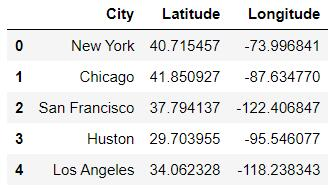
\includegraphics[width=0.5\textwidth]{c1.jpg}
\centering
\end{figure}

Some example resulting venues are:
\begin{figure}[h!]
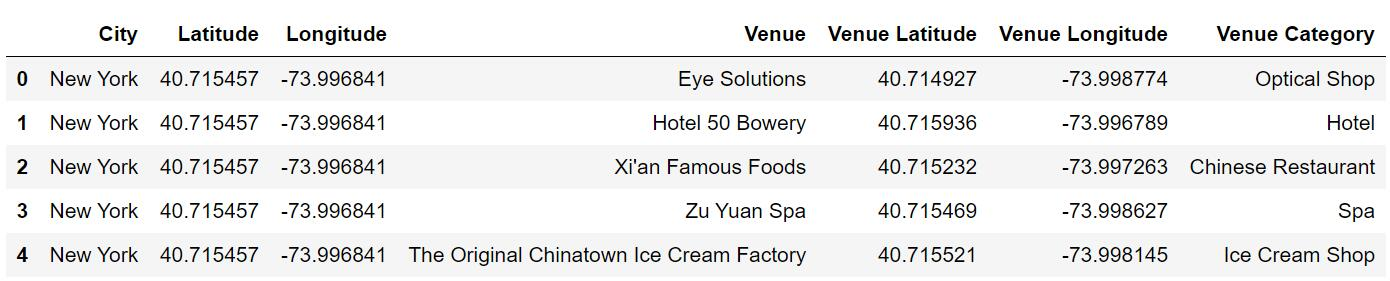
\includegraphics[width=1.0\textwidth]{c2.jpg}
\centering
\end{figure}

In total, 429 venues are selected around these 5 Chinatown, those data will tell us what defines a Chinese district.

\newpage

The data will be grouped by the city name, and encoded in terms of the venue category. Examples look like:
\begin{figure}[h!]
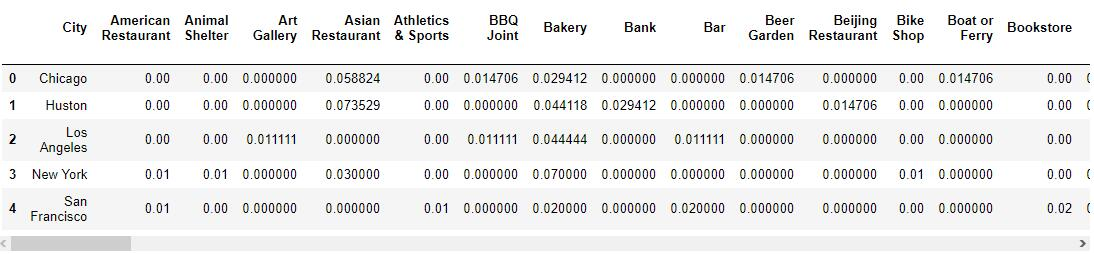
\includegraphics[width=1.0\textwidth]{c2_1.jpg}
\centering
\end{figure}

\subsection{Target City Data}

For data 2, the situation is more complicated.
For each target city, the data sources of neighborhoods vary, making the web-scraping work city-specific.
Here I choose a simple alternative approach.
For each input coordinates user interested, we generate a grid around that latitude and longitude coordinate, and analyze the target city based on this grid partition.
Here I take Charlotte, NC as an example to show how this approach works.

We select two points on google map to select areas include most of the metropolitan area of Charlotte, then the grid is constructed by equally partition 20$\times$20 sample coordinates within the selected area.
\begin{figure}[h!]
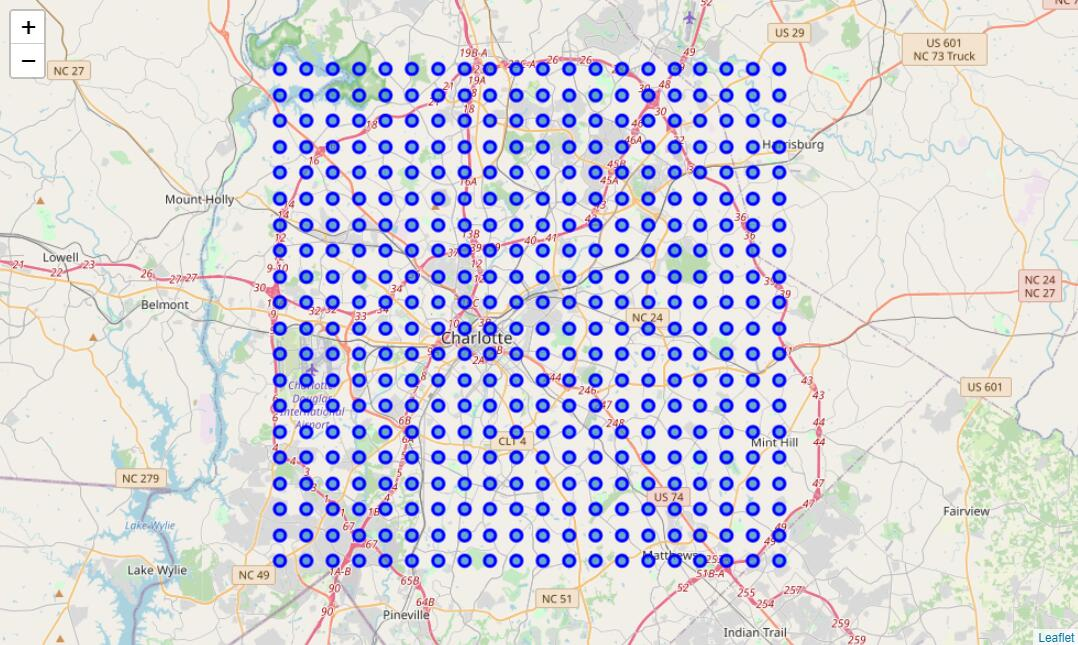
\includegraphics[width=1.0\textwidth]{c3.jpg}
\centering
\end{figure}

Then we loop over those coordinates and find venues within a certain radius of each point. Note that we will make that radius slightly larger than the half-distance of the two diagonal grid points to make sure that no venues are ignored.
In the Charlotte case, the radius is 1500 m.
By taking this approach, there will also have overlapping venues, where same venues appear in different grid points.
Since the grid points can locate in sparsely populated areas, where the number of venues is very small, I will ignore them to avoid potential statistical problems. Only grid points with over 15 venues will be appended into the data.

Example venues look like:
\begin{figure}[h!]
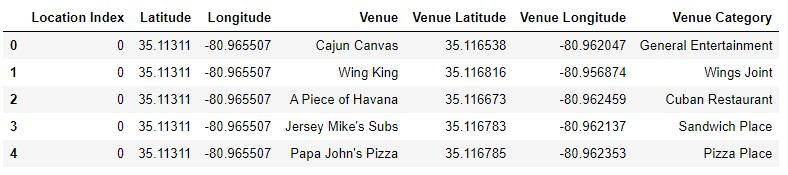
\includegraphics[width=1.0\textwidth]{c4.jpg}
\centering
\end{figure}

In total, 10041 venues are selected. Those data are where we want to get insight from.

Here I show another example to prove the workflow.
Find Atlanta on google map, and select the 
Input point 1 is $33.620260, -84.543165$, point 2 is $34.024354, -84.112095$, and the sample size is 20$\times$20:
\begin{figure}[h!]
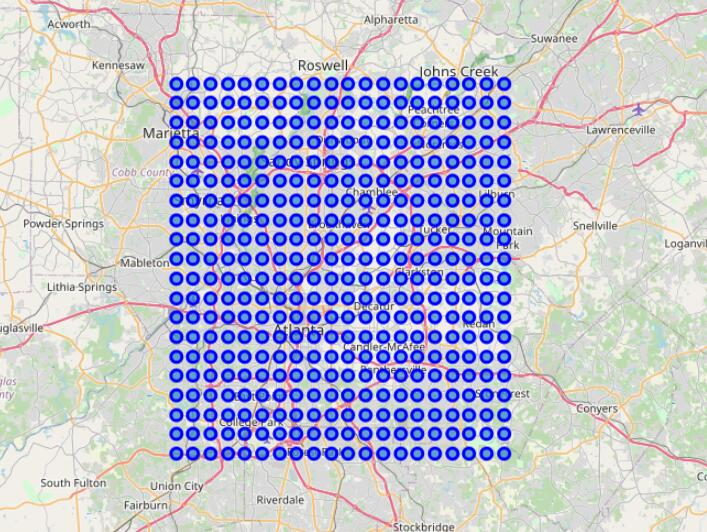
\includegraphics[width=1.0\textwidth]{c5.jpg}
\centering
\end{figure}

\newpage

The data will be grouped by grid point index, and encoded in terms of the venue category. Examples look like:
\begin{figure}[h!]
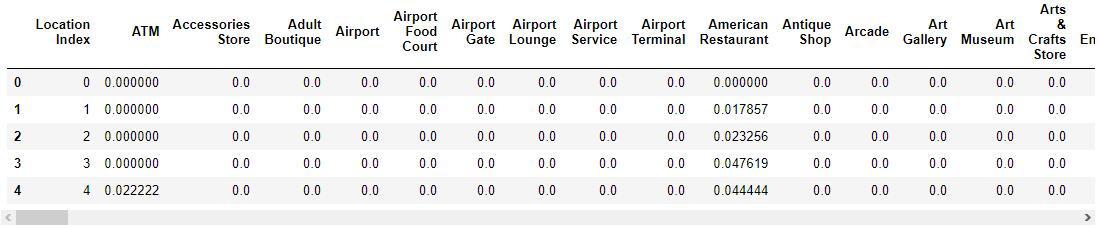
\includegraphics[width=1.0\textwidth]{c6.jpg}
\centering
\end{figure}

Then the data are ready to be analyzed.

\subsection{Usage of the Data}

The simplest idea is to use the unsupervised learning techniques only based on the target city data.
In this case, we do not need data 1.
However, Chinese venues are not common features for many US cities, it is very possible that naive unsupervised learning techniques cannot distinguish the Chinese district from other districts.
Therefore, the data 1 will play an important role to screen the venue types, and possibly introduce a weighted distances during the unsupervised learning.

\section{Methodology}
\subsection{Naive K-means Clustering}

\subsection{Feature Analysis}

\subsection{Weighted Distance K-means}

\section{Result and Discussion}

\subsection{Results of Charlotte and Atlanta}

\subsection{The Pipeline}

\subsection{Potential Problems}

\section{Conclusion}

\newpage

\bibliographystyle{unsrt}
\bibliography{capstone}

\end{document}
